%!TEX root = ../thesis.tex
%******************************************************************************
\chapter{An Adaptive Middleware for Near-Time Processing of Bulk Data}\label{ch:adaptive_middleware}
%******************************************************************************

\section{Introduction}\label{sec:introduction}

It has been shown in the previous Chapter \ref{ch:performance_evaluation}, that the end-to-end latency can be decreased by using a message-based processing style which facilitates single-event processing. While this approach is able to deliver near-time processing, it is hardly capable for bulk data processing due to the additional communication overhead for each processed message. In contrast, the batch processing style delivers high throughput but cannot provide near-time processing of data.

The processing type is usually a fixed property of an enterprise system that is decided when the architecture of the system is designed, prior to implementing the system. This choice depends on the non-functional requirements of the system. These requirements are not fixed and can change during the lifespan of a system, either anticipated or not anticipated.

Additionally, enterprise systems often need to handle load peaks that occur infrequently. For example, think of a billing system with moderate load over most of the time, but there are certain events with very high load such as New Year's Eve. Most of the time, a low end-to-end latency of the system is preferable when the system faces moderate load. During the peak load, it is more important that the system can handle the load at all. A low end-to-end latency is not as important as an optimized maximum throughput in this situation.

The results presented in the previous Chapter \ref{ch:performance_evaluation} show that throughput and latency depend on the granularity of data that is being processed. Additionally, the current throughput and latency also depend on the current load of the system. If the system is not able to handle the current load, messages are congested in the input queue which increases the latency of the system. A higher maximum throughput would decrease the latency in this case. The aggregation size used by the messaging system should depend on the current load of the system.

This chapter introduces the concept of an adaptive middleware which is able to adapt its processing type fluently between batch processing and single-event processing. It continuously monitors the load of the system and controls the message aggregation size. Depending on the current aggregation size, the middleware automatically chooses the appropriate service implementation and transport mechanism to further optimize the processing.

In this chapter, a solution to this problem is proposed:

\begin{itemize}
	\item The concept of a middleware is presented that is able to adapt its processing type fluently between batch processing and single-event processing. By adjusting the data granularity at runtime, the system is able to minimize the end-to-end latency for different load scenarios.
	\item A prototype has been built to evaluate the concepts of the adaptive middleware.
	\item A performance evaluation has been conducted using this prototype to evaluate the proposed concept of the adaptive middleware.
\end{itemize}

The remainder of this chapter is organized as follows. 

Section \ref{sec:ch04_requirements} describes the requirements of an adaptive middleware derived from the results of Chapter \ref{ch:performance_evaluation}. Section \ref{sec:ch05_middleware_concepts} introduces the core concepts of the \emph{Adaptive Middleware for Bulk Data Processing}. These concepts are implemented by components of the adaptive middleware that are described in Section \ref{sec:ch05_middleware_components}. There are several architectural design aspects that need to be considered to implement a system based on the adaptive middleware, which are discussed in Section \ref{sec:ch05_design_aspects}. To evaluate the concepts of the adaptive middleware, a prototype has been built. The design and implementation of this prototype is outlined in Section \ref{sec:ch05_prototype}. The prototype has been evaluated in Section \ref{sec:ch05_evaluation}. Section \ref{sec:ch5_related_work} gives an overview of other work related to this research. Finally, Section \ref{sec:ch5_summary} concludes this chapter.

\section{Requirements}
\label{sec:ch04_requirements}

The \emph{Adaptive Middleware} should implement the following requirements, which have been derived from the results of the performance analysis, as described in Chapter \ref{ch:performance_evaluation}:

\begin{itemize}
	\item \textbf{REQ1}: Message aggregation\\
	Aggregation of single messages or events
	\item \textbf{REQ2}: Aggregation strategies\\
	Support for different aggregation strategies, statically or dynamically at run-time
	\item \textbf{REQ3}: Message routing\\
	Messages should be routed to the appropriate service to allow for optimized processing depending on their aggregation size.
	\item \textbf{REQ4}: Monitoring\\
	Monitoring of current throughput, end-to-end latency and load of the system
	\item \textbf{REQ5}: Dynamic control of aggregation size\\
	Dynamic control of the aggregation size of the processed events at run-time depending on the current load of the system
\end{itemize}

\section{Middleware Concepts}
\label{sec:ch05_middleware_concepts}
Based on the requirements, as discussed in the previous section, this section describes the core concepts of the adaptive middlware: 
\begin{inparaenum}[(1)]
	\item message aggregation,
	\item message routing, and
	\item monitoring and control.
\end{inparaenum}

\subsection{Message Aggregation}
\label{sec:ch05_aggregator}
Message aggregation or batching of messages is the main feature of the adaptive middleware to provide a high maximum throughput.
The aggregation of messages has the following goals:

\begin{itemize}
	\item To decrease the overhead for each processed message
	\item To facilitate optimized processing
\end{itemize}

There are different options to aggregate messages, which can be implemented by the Aggregator:

\begin{itemize}
	\item \textbf{No correlation}: Messages are aggregated in the order in which they are read from the input message queue. In this case, an optimized processing is not simply possible.
	\item \textbf{Technical correlation:} Messages are aggregated by their technical properties, for example by message size or message format.
	\item \textbf{Business correlation}: Messages are aggregated by business rules, for example by customer segments or product segments.
\end{itemize}

Table \ref{table:ch05_aggregation_strategies} describes the advantages and disadadvantes of each aggregration strategy.

\begin{table}[htbp]
	\centering
	\begin{tabularx}{\textwidth}{@{} p{2cm} X X @{}}
		\caption{Properties of different aggregation strategies}\label{table:ch05_aggregation_strategies}\\
		\toprule
		\bfseries Aggregation Strategy & \centering\arraybackslash \bfseries Pro & \centering\arraybackslash \bfseries Con\\
		\midrule
		No correlation & \savespace
		\begin{titemize}
			\item Simple solution
			\item Even distribution of events
		\end{titemize} & \savespace
		\begin{titemize}
			\item optimization is not or hardly possible
		\end{titemize}\\
		\midrule
		Business correlation & \savespace
		\begin{titemize}
			\item Optimization is possible
		\end{titemize} & \savespace
		\begin{titemize}
			\item Analysation of processed data needed
			\item No even distribution of data (depending on correlation rule)
		\end{titemize}\\
		\midrule
		Technical correlation & \savespace
		\begin{titemize}
			\item Optimization is possible
		\end{titemize} & \savespace
		\begin{titemize}
			\item Analysation of processed data needed
			\item Rules can be defined after integration architecture
			\item No even distribution of data (depending on correlation rule), leads to uneven distribution of latency
		\end{titemize}\\
		\bottomrule
	\end{tabularx}
\end{table}

In Section \ref{sec:ch4_impact_granularity}, a static aggregation size has been used to optimize the latency and the throughput of a system.
This is not feasible for real systems, since the the latency and throughput also depends on the load of the system. Therefore, a dynamic aggregation size depending on the current load of the system is needed.

\subsection{Message Routing}
\label{sec:ch05_router}

The goal of the message routing is to route the message aggregate to the appropriate service, which is either optimized for batch or single event processing, to allow for an optimized processing. Message routing depends on how messages are aggegrated. Table \ref{table:ch05_message_routing} shows the different strategies of message routing.

\begin{table}[htbp]
	\centering
	\begin{tabularx}{\textwidth}{@{} p{3cm} X X @{}}
		\caption{Strategies for message routing}\label{table:ch05_message_routing}\\
		\toprule
		\bfseries Routing Strategy & \bfseries Examples & \bfseries Description\\
		\midrule
		Technical routing & \savespace
		\begin{titemize}
			\item Aggregation size
		\end{titemize} & Routing is based on the technical properties of a message aggregate.\\
		\midrule
		Content-based routing & \savespace
		\begin{titemize}
			\item Customer segments (e.g. business customers or private customers)
		\end{titemize} & Routing is based on the content of the message aggregate, that is, what type of messages are aggregated.\\
		\bottomrule
	\end{tabularx}
\end{table}

With high levels of message aggregation, it is not preferred to send the aggregated message payload itself over the message bus using Java Message Service (JMS) or SOAP. Instead, the message only contains a pointer to the data payload, which is transferred using File Transfer Protocol (FTP) or a shared database.

Message routing can be static or dynamic:
\begin{itemize}
	\item \textbf{Static routing:}\\ 
	Static routing uses static routic rules, that are not changed automatically.
	\item \textbf{Dynamic routing:}\\
	Dynamic routing adjusts the routing rules automatically at run-time, for example depending on \ac{QoS} properties of services. See for example \cite{Bai:2007aa}, \cite{Wu:2008aa} or \cite{Ziyaeva:2008aa}.
\end{itemize}

\subsection{Monitoring and Control}

\begin{figure}[htbp]
	\centering
	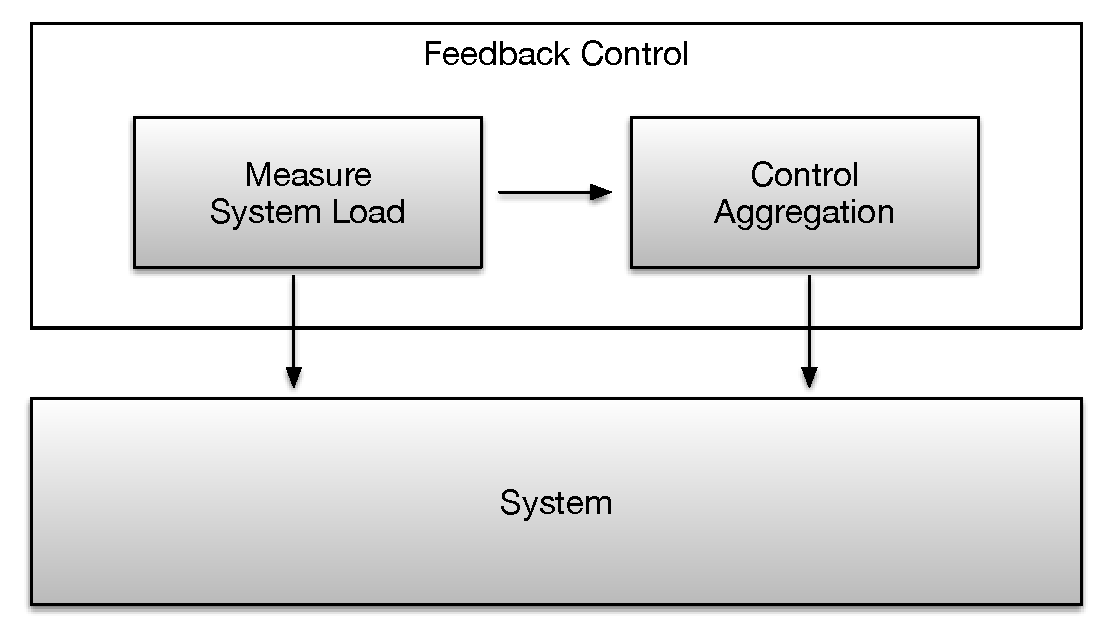
\includegraphics[width=\columnwidth]{ch05_monitoring_control}
	\caption{Monitoring and Control}
	\label{fig:ch05_monitoring_control}
\end{figure}

Aggregation size is not static, depends on the current load of the system:
\begin{itemize}
	\item If the current load of the system is low, aggregation size can be small to provide a low end-to-end latency of the system.
	\item If the current load of the system is high, aggregation size should be high to provide a high maximum throughput of the system. 
\end{itemize}

Monitoring component continuously monitors the the load of the system. 

To control the level of message aggregation at runtime, the adaptive middleware uses a closed feedback loop as shown in Figure \ref{fig:feedback_loop}.

\begin{itemize}
	\item Control Engineering Methodologies have been identified as a promising solution to implement self-adaptive software systems \citep{Patikirikorala:2012ky}, especially for performance control \citep{Abdelzaher:2003ea}.
	\item In particular, feedback loops provide generic mechanisms for self-adaption \citep{Brun:2009ww}. 
	\item Control engineering is based on control theory, which provides a systematic approach to designing closed loop systems that are stable, accurate, have short settling times, and do not overshoot \citep{Abdelzaher:2008ub}.
\end{itemize}

The feedback loop used by the adaptive middleware has the following properties:

\begin{itemize}
	\item \textbf{Input (u):} Current aggregation size
	\item \textbf{Output (y):} Change of queue size measured between sampling intervals
	\item \textbf{Set point (r):} The change of queue size should be zero.
\end{itemize}

Ultimately, we want to control the average end-to-end latency depending on the current load of the system. The change of queue size seems to be an appropriate quantity because it can be directly measured without a lag at each sampling interval, unlike for example the average end-to-end latency.

\begin{figure}[htbp]
	\centering
	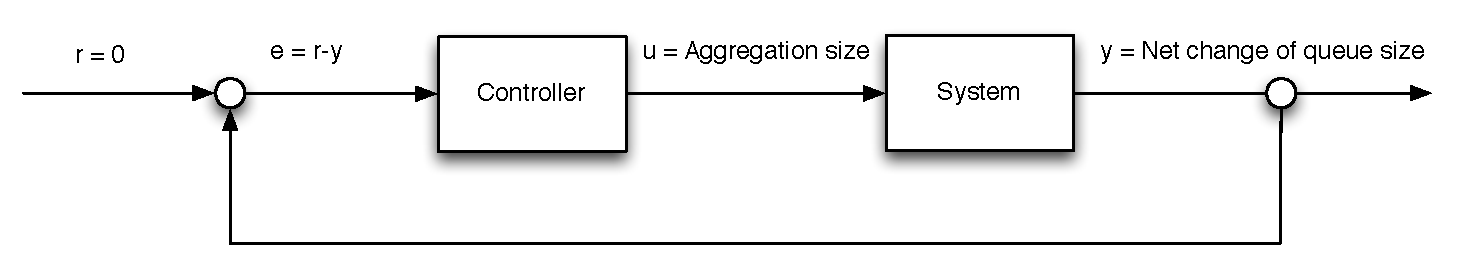
\includegraphics[width=\columnwidth]{feedback_loop}
	\caption{Feedback loop to control the aggregation size}
	\label{fig:feedback_loop}
\end{figure}

\section{Middleware Components}
\label{sec:ch05_middleware_components}
Table \ref{table:ch4_middleware_components} shows the components of the middleware, that are based on the Enterprise Integration Patterns described by \cite{Hohpe:2003fk}.

\begin{table}[htpb]
	\caption{Components of the Adaptive Middleware. We are using the notation defined by \cite{Hohpe:2003fk}}
	\label{table:ch4_middleware_components}
	\centering
	\begin{tabular}{|m{3cm}|m{2cm}|m{5cm}|}
		\hline
		\bfseries Symbol & \bfseries Component & \bfseries Description\\
		\hline 
		\begin{center}
			
\includegraphics[scale=0.5]{message_symbol}
		\end{center} 
		& Message & A single message representing a business event.\\
		\hline 
		\begin{center}
			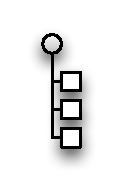
\includegraphics[scale=0.5]{aggregate_symbol} 
		\end{center}
		& Message Aggregate & A set of messages aggregated by the Aggregator component.\\
		\hline
		\begin{center}
			
\includegraphics[scale=0.5]{queue_symbol} 
		\end{center}
		& Queue & Storage component which stores messages using the \ac{FIFO} principle.\\
		\hline 
		\begin{center}
			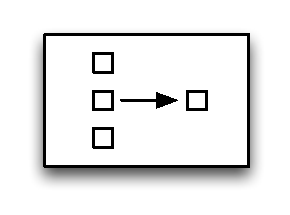
\includegraphics[scale=0.5]{aggregator_symbol}
		\end{center}
		& Aggregator & Stateful filter which stores correlated messages until a set of messages is complete and sends this set to the next processing stage in the messaging route.\\
		\hline
		\begin{center}
			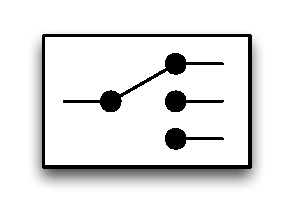
\includegraphics[scale=0.5]{router_symbol} 
		\end{center}
		& Router & Routes messages to the appropriate service endpoint, for example depending on the aggregation size of the message.\\
		\hline
		\begin{center}
			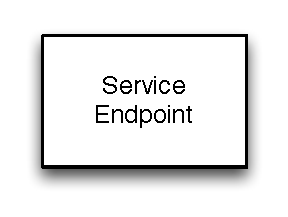
\includegraphics[scale=0.5]{endpoint_symbol} 
		\end{center}
		& Service Endpoint & Represents a business service.\\
		\hline
	\end{tabular}
\end{table}

\section{Design Aspects}
\label{sec:ch05_design_aspects}
This section describes aspects that should be taken into account when designing an adaptive system for bulk data processing.

\subsection{Usage Scenarios}
\todo[inline]{do we need this?}

\begin{itemize}
	\item different usage scenarios
	\item single aggregator, request/response integration pattern
	\item single aggregator, point to point channel
	\item system consisting of multiple subsystems, with each subsystem having an input queue, aggregator, router
\end{itemize}

\begin{landscape}
	\begin{figure*}[htpb]
		\centering
		\mbox{\subfloat[request/response integration pattern]{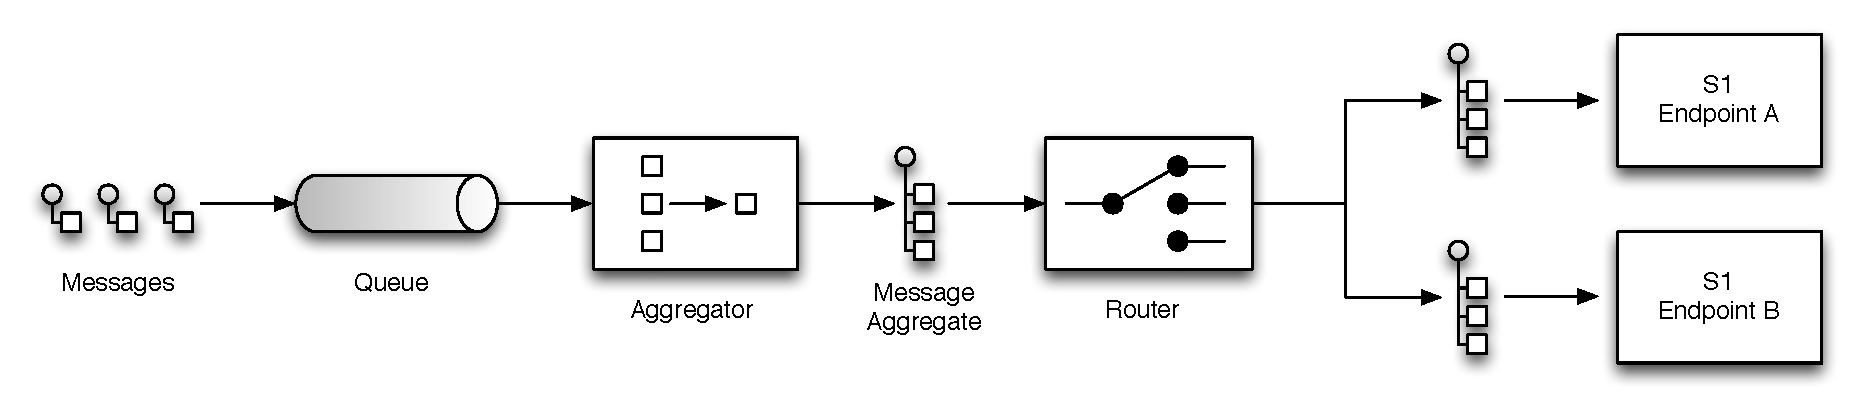
\includegraphics[scale=0.5]{ch5_usage_scenario_1}\label{fig:ch4_usage_scenario_1}}}
		\mbox{\subfloat[point-to-point channel integration pattern]{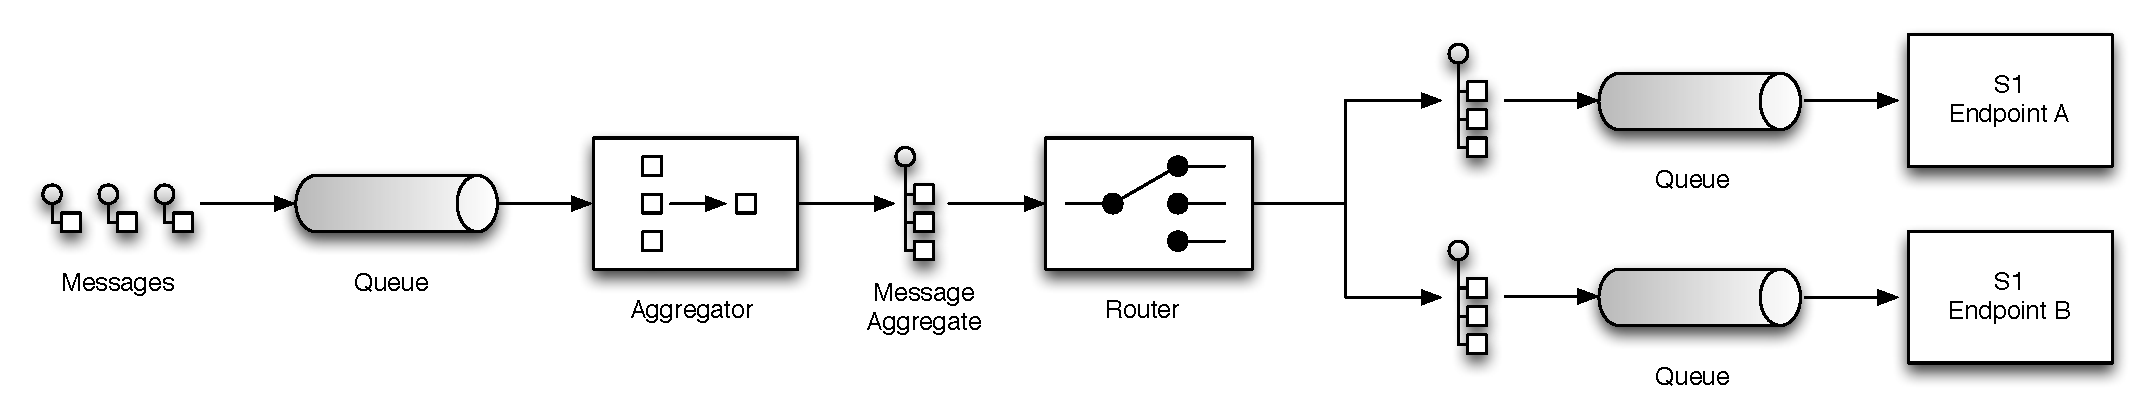
\includegraphics[scale=0.5]{middleware_components}}}
		\caption{Usage scenarios}
	\end{figure*}
\end{landscape}

\subsection{Service Design}
\label{sec:ch05_service_design}

The services that implement the business functionality of the system need to be explicitely designed to support the runt-time adaption between single-event and batch processing. 

There are different options for the design of these services:
\begin{itemize}
	\item Single Service interface with distinct operations for single and batch processing
	\begin{itemize}
		\item The service provides different distinct operations for high and low aggregation sizes with optimized implementations for batch and single-event processing. The decision which operation should be called is done by the message router. It is generally not possible to use different transports for different aggregation sizes.
	\end{itemize}
	\item Single Service interface with a single operation for both single and batch processing
	\begin{itemize}
		\item The service provides a single operation that is called for all aggregation sizes. The decision which optimization should be used is done by the service implementation. It is not possible to use different transports for different aggregation sizes.
	\end{itemize}
	\item Multiple service interfaces for single and batch processing (or different aggregation sizes)
	\begin{itemize}
		\item The logical business service is described by distinct service interfaces which contain operations for either batch processing or single-event processing. The decision which operation should be called is done by the message router. It is possible to use different transports for different aggregation sizes.
	\end{itemize}
\end{itemize}

The choice of service design relates to where you want to have the logic for the message routing for optimized processing. With a single service offering distinct operations for single-event and batch processing, as well as with distinct service for each processing style, the message router decides which service endpoint should be called. In contrast, using a single service with a single operation for both processing styles, the service itself is responsible for choosing the appropriate processing strategy. Using a different integration type for each processing style is not possible in this case.

Table \ref{table:ch05_service_design} shows the advantages and disadvantages for each service design option.

Listing \ref{listing:ch5_service_design_if} shows the interface of a service offering different operations for batch processing (line 6) and single-event processing (line 10).

\begin{lstlisting}[caption={Java interface of a web  service offering different operations for single and batch processing.},label=listing:ch5_service_design_if]
	@WebService
	@SOAPBinding(style=Style.DOCUMENT, use=Use.LITERAL, parameterStyle=ParameterStyle.WRAPPED)
	public interface RatingPortType {
		@WebMethod(operationName="processCallDetails")
		@WebResult(name="costedEvents")
		public Costedevents processCallDetails(@WebParam(name="callDetailRecords") SimpleCDRs callDetailRecords) throws ProcessingException, Exception;
	
		@WebMethod(operationName="processCallDetail")
		@WebResult(name="costedEvent")
		public Costedevent processCallDetail(@WebParam(name="simpleCDR") SimpleCDR callDetailRecord) throws ProcessingException, Exception;
	}
\end{lstlisting}

\begin{table}[htpb]
	\centering
	\begin{tabularx}{\textwidth}{@{} X X X @{}}
		\caption{Options for designing service interfaces}\label{table:ch05_service_design}\\
		\toprule
		\bfseries Interface option & \bfseries Pros & \bfseries Cons\\
		\midrule
		Single service /\\distinct Operations & \savespace
		\begin{titemize}
			\item Lorem ipsum
		\end{titemize} & \savespace
		\begin{titemize}
			\item Lorem ipsum
		\end{titemize}\\
		\midrule
		Single service /\\single operation & \savespace
		\begin{titemize}
			\item 
		\end{titemize} & \savespace
		\begin{titemize}
			\item Lorem ipsum
		\end{titemize}\\
		\midrule
		Distinct services & \savespace
		\begin{titemize}
			\item
		\end{titemize} & \savespace
		\begin{titemize}
			\item Lorem ipsum
		\end{titemize}\\
		\bottomrule
	\end{tabularx}
\end{table}

\subsection{Integration and Transports}
\label{sec:ch05_transports}
The integration architecture defines the technologies that are used to integrate the business services. In general, different integration styles with different transports are used for batch processing and single-event processing, which needs to be taken into account when designing an adaptive system for bulk data processing (Please refer to Section \ref{sec:batch_processing} and \ref{sec:message_processing} for a detailed description of each processing style).

When using high aggegration sizes, it is not feasible to use the same transports as with low aggregation sizes. Large messages should not be transferred over the messaging system. Instead, a file based transport using \ac{FTP} or database-based integration should be used. When using a messaging system, the payload of large messages should not be transported over the messaging system. For example by implementing the \emph{Claim Check} \ac{EIP} (refer to Section \ref{sec:ch03_eip} for a detailed description of this pattern). Table \ref{table:ch05_transports} summarizes the transport options for low and high aggregation sizes.

\begin{table}[htbp]
	\centering
	\begin{tabularx}{\textwidth}{@{} X X X @{}}
		\caption{Transport options for high and low aggregation sizes}\label{table:ch05_transports}\\
		\toprule
		\bfseries Aggregation Size & \bfseries Transport Options\\
		\midrule
		High & \savespace
		\begin{titemize}
			\item Database
			\item File-based (e.g. \ac{FTP})
			\item Claim Check \ac{EIP}
		\end{titemize}\\
		\midrule
		Low & \savespace
		\begin{titemize}
			\item \ac{JMS}
			\item SOAP
		\end{titemize}\\
		\bottomrule
	\end{tabularx}
\end{table}

Additionally, the technical data format should be considered. 

The concrete threshold between low and high aggregation sizes depends on the integration architecture and implementation of the system, such as the integration architecture and the deployed messaging system.

The choice of the appropriate integration transport for a service is implicitly implemented by the message router (see Section \ref{sec:ch05_router}).

\subsection{Error Handling}

Message aggregation has also an impact on the handling of errors that occur during the processing. Depending on the cause of the error, there are two common types of errors: 
\begin{itemize}
	\item \textbf{Technical errors}\\
	Technical errors are errors caused by technical reasons, for example an external system is not availaible or does not respond within a certain timeout or the processed message has an invalid format.
	\item \textbf{Business errors}\\
	Business errors are caused by violation of business rules, for example a call detail record contains a tariff that is no longer valid.
\end{itemize}

The following points should be taken into account, when designing the error handling for an adaptive system for bulk data processing:
\begin{itemize}
	\item Write erroneous messages to an error queue for later processing. 
	\item Use multiple queues for different types of errors, for example distinct queues for technical and business errors to allow different strategies for handling them. Some type of errors can be fixed automatically, for example an error that is caused by an outage of an external system, while other errors need to be fixed manually.
	\item If the erroneous messages is part of an aggregated message, it should be extracted from the aggregate to prevent the whole aggregate from beeing written to the error qeue, especially when using high aggregation sizes.
\end{itemize}

\subsection{Controller Design}
\label{sec:ch05_controller_design}

There are several approaches for the implementation of feedback-control system. \cite{Hellerstein:2004a} describe two major steps:
\begin{enumerate}
	\item modeling the dynamics of the system
	\item developing a control system
\end{enumerate}

There are different approaches that are used in practice to model the dynamics of a system \citep{Hellerstein:2004tu}:
\begin{itemize}
	\item Empirical approach using curve fitting to create a model of the system
	\item Black-box modeling
	\item Modeling using stochastic approaches, especially queuing theory
	\item Modeling using special purpose representations, for example the first principles analysis
\end{itemize}

The following approach has been taken in this research:

\begin{enumerate}
	\item Define the control problem
	\item Define the input and output variables of the system
	\item Measure the dynamics of the system
	\item Create a model of the system
	\item Develop the control system
\end{enumerate}

\subsubsection{Control Problem}

\begin{itemize}
	\item Control problem: minimise the end-to-end latency of the system by controlling the message aggregation size
	\item aggregation size used by the messaging system should depend on the current load of the system
	\item when system faces high load, aggregation sizes should be increased
	\item when sytem faces low load, aggregation sizes could be decreases
\end{itemize}
\subsubsection{Input/Output Signals}

\cite{Janert:2013aa} describes the following criteria for selecting input control signals:
\begin{itemize}
	\item \textbf{Availability}\\
	It should be possible to influence the control input directly and immediately.
	\item \textbf{Responsiveness}\\
	The system should respond quickly to a change of the input signal. Inputs whose effect is subject to latency or delays should be avoided when possible.
	\item \textbf{Granularity}\\
	It should be possible to adjust the control input in small increments. If the control input can only be adjusted in fixed increments, then it could be necessary to consider this in the controller or actuator implementation.
	\item \textbf{Directionality}\\
	How does the control input impact the control output? Does an increased control input result in increased or decreased output?
\end{itemize}

Additionally, the following criteria should be considered for selecting output control signals:

\begin{itemize}
	\item \textbf{Availability}\\
	The quantity must be observable without gaps and delays.
	\item \textbf{Relevance}\\
	The output signal should be relevant for the behaviour of the system that should be controlled. 
	\item \textbf{Responsiveness}\\
	The output signal should reflect changes of the state of the system quickly without lags and delays.
	\item \textbf{Smoothness}\\
	The output signal should be smooth and does not need to be filtered.
\end{itemize}

With regard to these criteria, the following input and output control signals have been choosen 
\begin{itemize}
	\item \textbf{Input (u):} Current aggregation size
	\item \textbf{Output (y):} Change of queue size measured between sampling intervals
	\item \textbf{Set point (r):} The change of queue size should be zero.
\end{itemize}

\subsubsection{Control Strategy}
\label{sec:ch05_control_strategy}

\paragraph{Simple controller}\mbox{}\\
A simple control strategy could be implemented as follows:
\begin{itemize}
	\item change queue > 0: Increase the aggregation size by a certain amount
	\item change queue = 0: Do nothing
\end{itemize}

\paragraph{PID controller}\mbox{}\\
Another option would be to use a standard PID-Controller instead, which calculates the output value $u_k$ at time step $k$ of the controller depending on the current (proportional part), previous (integral part) and expected future error (differential part):
\begin{displaymath}
	u_k=K_p*e_k+K_i*T_a\sum_{i=0}^k e_i+\frac{K_d}{T_a}(e_k-e_{k-1})
\end{displaymath}
with $K_p$ being the controller gain of the proportional part, $e_k$ being the error ($r-y$) at step $k$, $K_i$ being the controller gain of the integral part, $T_a$ being the sampling interval and $K_d$ being the controller gain of the differential part.

\section{Prototype Implementation}
\label{sec:ch05_prototype}

This section describes the implementation of the prototype which implements the core concepts of the adaptive middleware. The prototype is based on the messaging prototype described in Section \ref{sec:ch04_messaging_prototype}.

The prototype extends the messaging prototype with the following components (see Figure \ref{fig:ch05_components_prototype}):
\begin{itemize}
	\item \textbf{Performance Monitor}\\
	The \emph{Performance Monitor} manages the feedback-control loop by periodically calling the \emph{Sensor} and updating the \emph{Controller}. Additionally, it calculates the current throughput and end-to-end latency of the sytem.
	\item \textbf{Sensor}\\
	The \emph{Sensor} is responsible for getting the current size of the message queue using \ac{JMX}.
	\item \textbf{Controller}\\
	The \emph{Controller} calculates the new value for the aggregation size base on the setpoint and the current error.
	\item \textbf{Actuator}\\
	The \emph{Actuator} is responsible for setting the new aggregation size of the \emph{Aggregator} calculated by the \emph{Controller}.
\end{itemize}

\begin{figure}[htbp]
	\centering
	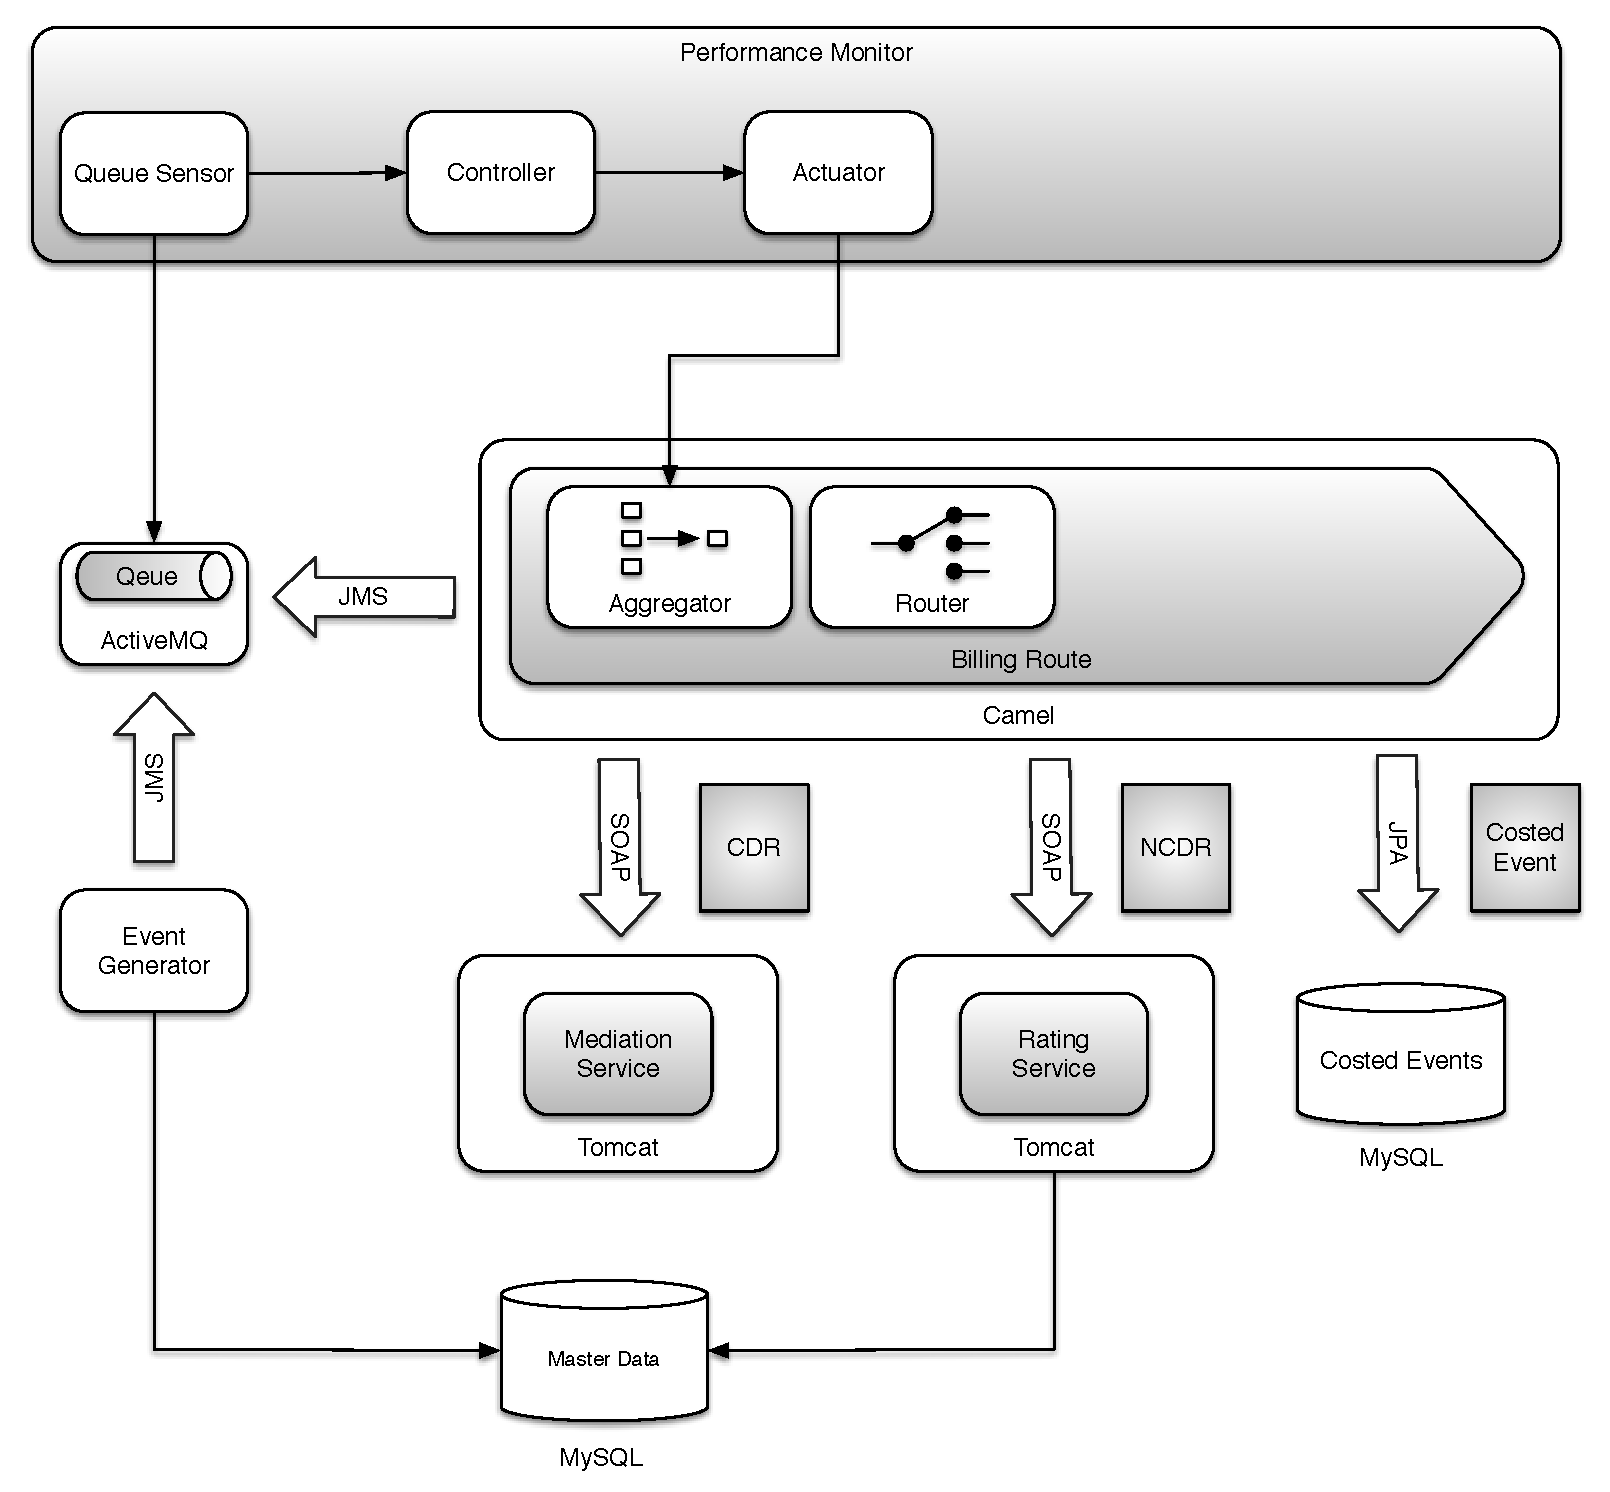
\includegraphics[width=\columnwidth]{ch05_components_prototype}
	\caption{Components of the prototype system}
	\label{fig:ch05_components_prototype}
\end{figure}

\subsection{Aggregator}
The message aggregator uses the same \emph{AggregationStrategy} as the messaging prototype as described in Section \ref{sec:ch4_impact_granularity}, as shown in Listing \ref{listing:ch5_UsageEventsAggrationStrategy}:
\begin{itemize}
	\item The \emph{aggregate} method, which is called by the aggregator for each message, takes two arguments: \emph{oldExchange} contains the already aggregated messages, \emph{newExchange} contains the new arrived message (line 4).
	\item If there are not yet any aggregated messages stored in the aggregator (line 5):
	\begin{itemize}
		\item The message body (\emph{rawUsageEvent}) is read from the new arrived message (line 6).
		\item A new \emph{usageEventsList} is generated (line 8).
		\item The message body is added to the list and the list is added to the incoming message, which now becomes the new message aggregate.
	\end{itemize}
	\item Otherwise, the message body of the new message is added to list of the aggregated messages (line 22).
\end{itemize}

\begin{lstlisting}[caption={UsageEventsAggrationStrategy},label=listing:ch5_UsageEventsAggrationStrategy]
public class UsageEventsAggrationStrategy implements AggregationStrategy {

	@Override
	public Exchange aggregate(Exchange oldExchange, Exchange newExchange) {
		if (oldExchange == null) {
			RawUsageEvent rawUsageEvent = newExchange.getIn().getBody(RawUsageEvent.class);
			RawUsageEvents rawUsageEvents = new RawUsageEvents();
			List<RawUsageEvent> usageEventList = new ArrayList<RawUsageEvent>();
			rawUsageEvents.setUsageEvents(usageEventList);
			usageEventList.add(rawUsageEvent);
			newExchange.getIn().setBody(rawUsageEvents);
			increaseAggregateSize(newExchange);
			
			Long startTime = getStartTime(newExchange);
			addStartTime(newExchange, startTime);
			
			return newExchange;
		}
		else {
			RawUsageEvents rawUsageEvents = oldExchange.getIn().getBody(RawUsageEvents.class);
			RawUsageEvent rawUsageEvent = newExchange.getIn().getBody(RawUsageEvent.class);
			rawUsageEvents.getUsageEvents().add(rawUsageEvent);
			increaseAggregateSize(oldExchange);
			
			Long startTime = getStartTime(newExchange);
			addStartTime(oldExchange, startTime);
			
			return oldExchange;
		}
	}
	
	//Additional methods removed for simplification...
	
}
\end{lstlisting}

The aggregator is configured to dynamically use the aggregation size (\emph{completionSize}) set by a message header, as shown in Listing \ref{listing:ch5_aggregator_definition} (line 2). This message header is set by the \emph{Actuator} (see Section \ref{sec:ch05_actuator}), which is controlled by the \emph{Controller} (see Section \ref{sec:ch05_controller}).

\begin{lstlisting}[caption={Aggregator configuration in definition of BillingRoute},label=listing:ch5_aggregator_definition]
.aggregate(constant(true), new UsageEventsAggrationStrategy())
	.completionSize(header(completionSizeHeader))
	.completionTimeout(completionTimeout)
	.parallelProcessing()
\end{lstlisting}

\subsection{Feedback-Control Loop}

Figure \ref{fig:ch05_components_feedback_loop} shows the components of the feedback-control loop.

\begin{figure}[htbp]
	\centering
	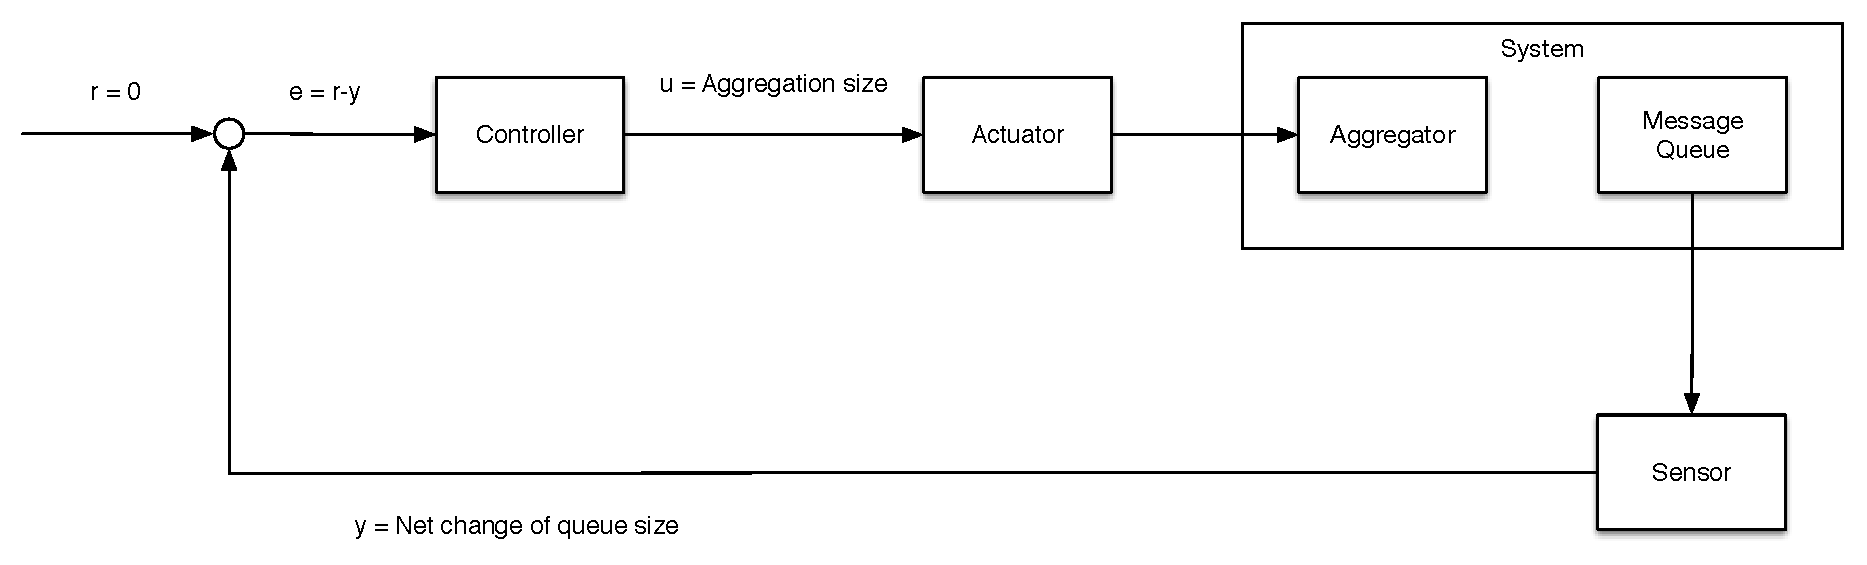
\includegraphics[width=\columnwidth]{ch05_components_feedback-loop}
	\caption{Components of the feedback-control loop}
	\label{fig:ch05_components_feedback_loop}
\end{figure}

\subsubsection{Sensor}

The \emph{JmxSensor} implements the \emph{Sensor} interface (see Figure \ref{fig:ch05_classdiagram_sensor}). It reads the current length of the input queue of the \emph{ActiveMQ} server instance using \ac{JMX}.

\begin{figure}[htbp]
	\centering
	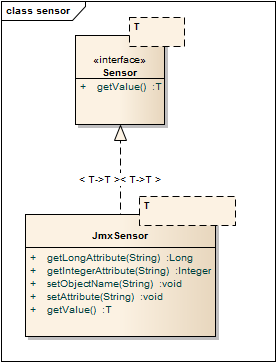
\includegraphics[scale=0.6]{ch05_classdiagram_sensor}
	\caption{\ac{UML} classdiagram showing the sensor classes}
	\label{fig:ch05_classdiagram_sensor}
\end{figure}

\subsubsection{Controller}
\label{sec:ch05_controller}
A \emph{Controller} has to implement the \emph{Controller} interface. The following implementations of the \emph{Controller} interface have been implemented (see Figure \ref{fig:ch05_classdiagram_controller}):
\begin{itemize}
	\item \textbf{BasicController}\\
	Implements a generic controller. The control strategy is provided by an implementation of the \emph{ControllerStratey}.
	\item \textbf{TestController}\\
	A controller used for testing the static behaviour of the system.
\end{itemize}

\begin{figure}[htbp]
	\centering
	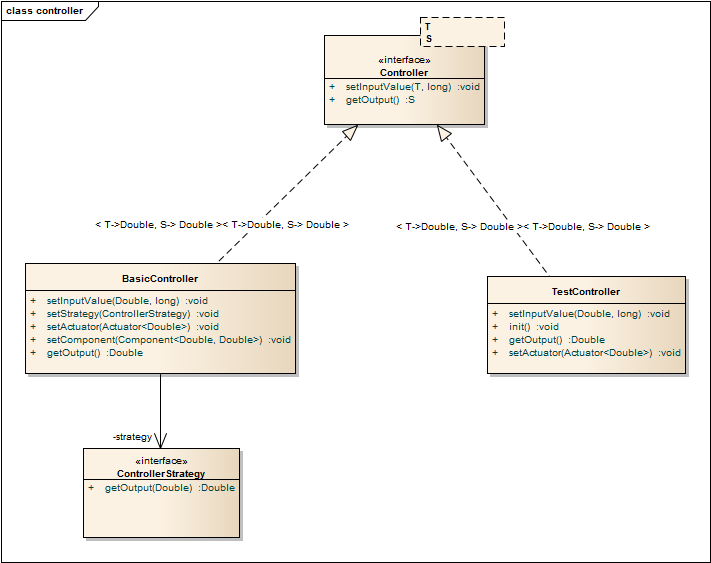
\includegraphics[width=\columnwidth]{ch05_classdiagram_controller}
	\caption{\ac{UML} classdiagram showing the controller classes}
	\label{fig:ch05_classdiagram_controller}
\end{figure}

The strategy of the controller is implemented by a \emph{Controller Strategy} which implements the \emph{ControllerStrategy} interface (see Listing \ref{listing:ch5_controller_strategy}).

\begin{lstlisting}[caption={ControllerStrategy Interface},label=listing:ch5_controller_strategy]
package com.jswiente.phd.performance.controller;

public interface ControllerStrategy {
	public Double getOutput(Double error);
}
\end{lstlisting}

Figure \ref{fig:ch05_classdiagram_controllerStrategy} shows the available implementations of the \emph{ControllerStrategy}.

\begin{figure}[htbp]
	\centering
	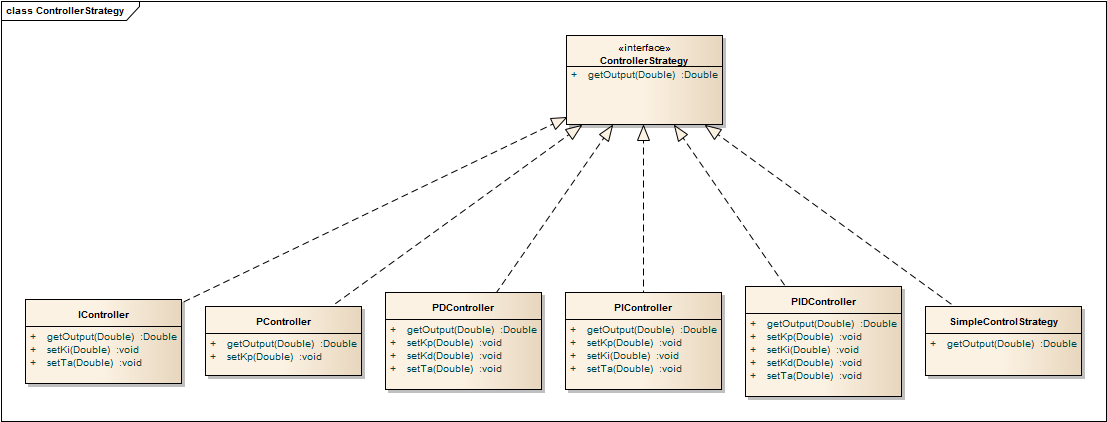
\includegraphics[width=\columnwidth]{ch05_classdiagram_controllerStrategy}
	\caption{\ac{UML} classdiagram showing the controller strategy classes}
	\label{fig:ch05_classdiagram_controllerStrategy}
\end{figure}

\paragraph{Simple Controller}\mbox{}\\

Listing \ref{listing:ch5_simple_controller} shows the implementation of the simple control strategy, as described in Section \ref{sec:ch05_control_strategy}:
\begin{itemize}
	\item If the queue size increases, increase the aggregation size (line 10-13).
	\item Otherwise, do not change the aggregation size (line 22).
	\item Periodically decrease the aggregation size by one (line 17-20).
\end{itemize}

\begin{lstlisting}[caption={Implementation of the simple control strategy},label=listing:ch5_simple_controller]
public class SimpleControlStrategy implements ControllerStrategy {

	@Value("${simpleController.period1}")
	private int period1;
	@Value("${simpleController.period2}")
	private int period2;
	private int timer = 0;
	
	public Double getOutput(Double error) {
		if (error > 0) {
			timer = period1;
			return +1.0;
		}

		timer--;
		
		if (timer == 0) {
			timer = period2;
			return -1.0;
		}
		
		return 0.0;
	}

}	
\end{lstlisting}

\paragraph{PID Controller}\mbox{}\\

The implementation of the \emph{PID Controller}, as described in Section \ref{sec:ch05_control_strategy} is straight forward, as shown in Listing \ref{listing:ch5_pid_controller}.

\begin{lstlisting}[caption={Implementation of PID Controller},label=listing:ch5_pid_controller]
public class PIDController implements ControllerStrategy {
	
	@Value("${controller.kp}")
	private Double kp;
	
	@Value("${controller.ki}")
	private Double ki;
	
	@Value("${controller.kd}")
	private Double kd;
	
	@Value("${controller.ta}")
	private Double ta;
	
	private Double errorSum = 0.0;
	private Double previousError = 0.0;

	public Double getOutput(Double error) {
		errorSum = errorSum + error;
		Double output = kp * error + ki * ta * errorSum + (kd * (error - previousError)/ta);
		previousError = error;
		return output;
	}

	//Setter methods removed for simplification...

}

\end{lstlisting}

\subsubsection{Actuator}
\label{sec:ch05_actuator}

The \emph{AggregateSizeActuator} is responsible for setting the aggregation size of the \emph{Aggregator} and is controlled by the \emph{Controller} (see Figure \ref{fig:ch05_classdiagram_actuator}).

\begin{figure}[htbp]
	\centering
	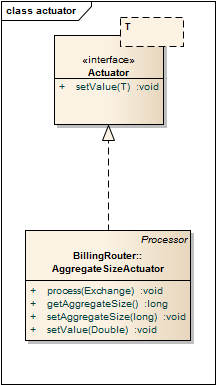
\includegraphics[scale=0.6]{ch05_classdiagram_actuator}
	\caption{\ac{UML} classdiagram showing the actuator classes}
	\label{fig:ch05_classdiagram_actuator}
\end{figure}

It \emph{AggregateSizeActuator} implements the \emph{Actuator} interface (see Listing \ref{listing:ch5_actuator_interface}). 

\begin{lstlisting}[caption={Actuator Interface},label=listing:ch5_actuator_interface]
package com.jswiente.phd.performance.actuator;

public interface Actuator<T> {

	public void setValue(T value);
}
\end{lstlisting}

The \emph{AggregateSizeActuator} sets the aggregation size (\emph{completionSize}) by setting a specific header in the currently processed message, as shown in Listing \ref{listing:ch5_aggregateSizeActuator} (line 15). 

\begin{lstlisting}[caption={AggregateSizeActuator},label=listing:ch5_aggregateSizeActuator]
@Component
public class AggregateSizeActuator implements Processor, Actuator<Double> {

	@Value("${camel.aggregator.completionSize}")
	private long aggregateSize;
	
	@Value("${camel.aggregator.completionSizeHeader}")
	private String completionSizeHeader;
	
	private static final Logger logger = LoggerFactory
			.getLogger(AggregateSizeActuator.class);
	
	@Override
	public void process(Exchange exchange) throws Exception {
		exchange.getIn().setHeader(completionSizeHeader, aggregateSize);
	}

	@ManagedAttribute
	public long getAggregateSize() {
		return aggregateSize;
	}

	@ManagedAttribute
	public void setAggregateSize(long aggregateSize) {
		logger.debug("Setting aggregateSize to: " + aggregateSize);
		this.aggregateSize = aggregateSize;
	}

	@Override
	public void setValue(Double value) {
		logger.debug("Actuator: Setting aggregateSize to: " + value);
		long aggregateSize = Math.round(value);
		this.setAggregateSize(aggregateSize);
	}

}

\end{lstlisting}

\subsubsection{Performance Monitor}
The \emph{Performance Monitor} manages the feedback-control loop by periodically calling the \emph{Sensor} and updating the \emph{Controller}. Additionally, it calculates the current throughput and end-to-end latency of the sytem using the \emph{StatisticsService} (see Figure \ref{fig:ch05_classdiagram_monitor}).

\begin{figure}[htbp]
	\centering
	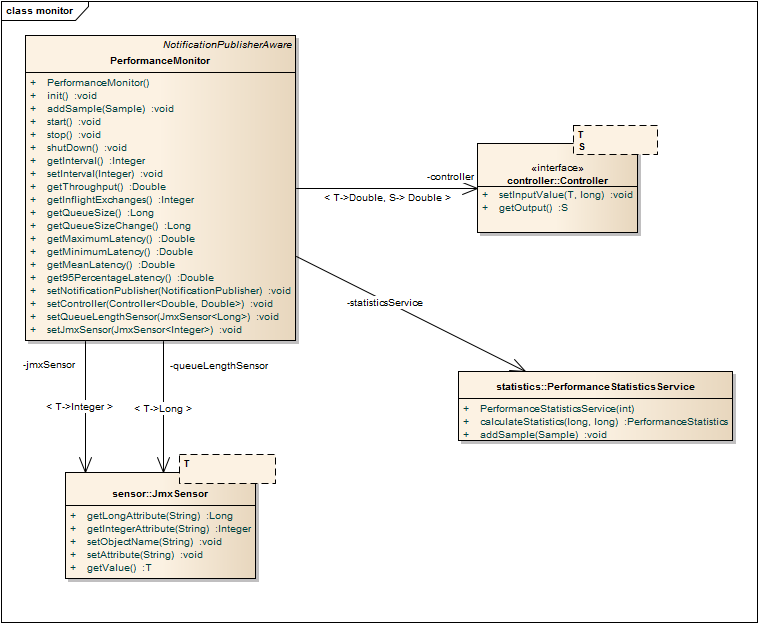
\includegraphics[width=\columnwidth]{ch05_classdiagram_monitor}
	\caption{\ac{UML} classdiagram showing the \emph{PerformanceMonitor}}
	\label{fig:ch05_classdiagram_monitor}
\end{figure}

\subsection{Load Generator}

The \emph{Load Generator} is used to generate the system load by generating events (\acp{CDR}) and writing them to the the input message queue of the system. It is implemented as a stand-alone Java program using a command-line interface.

Figure \ref{fig:ch5_datagenerator_classdiagram} shows the \ac{UML} class diagram of the load generator.

\begin{figure}[htpb]
	\centering
	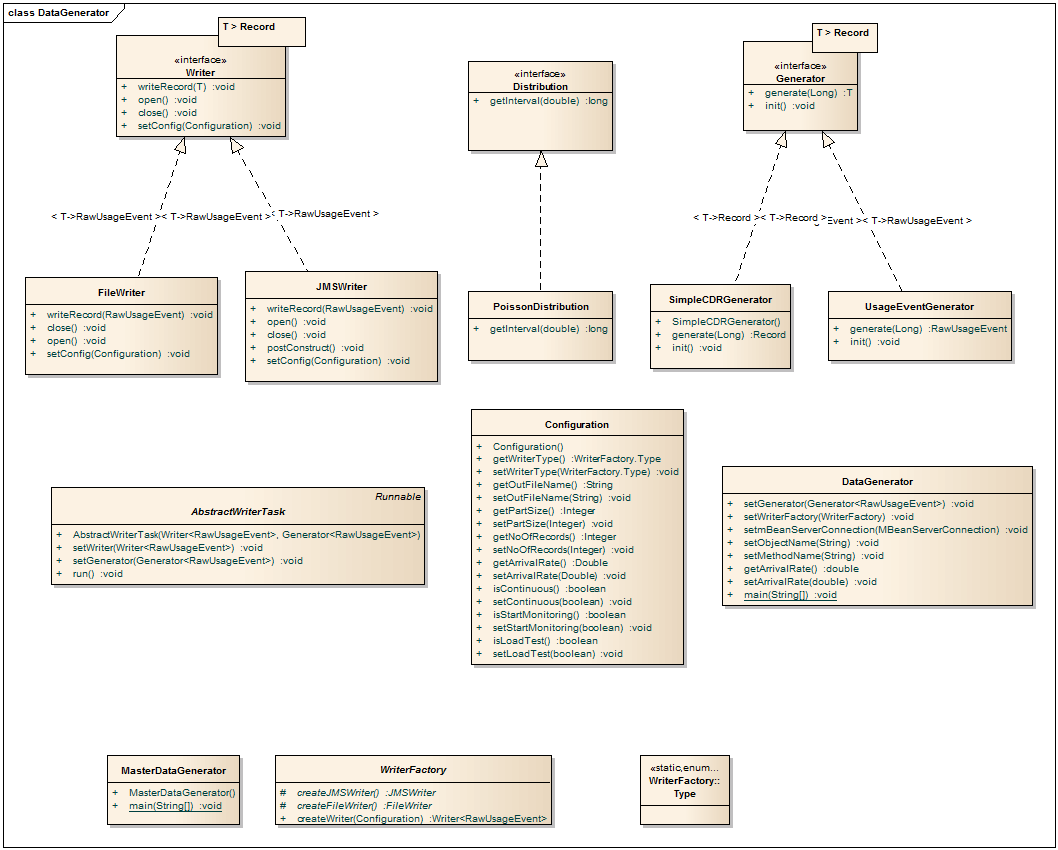
\includegraphics[width=\textwidth]{ch6_datagenerator_classdiagram}
	\caption{\ac{UML} class diagram of the \emph{Load Generator}}
	\label{fig:ch5_datagenerator_classdiagram}
\end{figure}

\begin{itemize}
	\item \textbf{DataGenerator}\\
	This is the main class of the \emph{DataGenerator}.
	\item \textbf{Writer}\\
	The \emph{Writer} interface defines methods for writing the generated events. There are two implementations available, the \emph{FileWriter}, which is used to write the generated to a file and the \emph{JmsWriter}, which is used to write the events to a \ac{JMS} queue.
	\item \textbf{Generator}\\
	The \emph{Generator} interface defines methods for generating events.  
	\item \textbf{Distribution}\\
	The \emph{Distribution} interface represents an event distribution used by the \emph{DataGenerator}. The \emph{PoissonDistribution} is the single implementation of this interface.
	\item \textbf{Configuration}\\
	This class holds a specific set of configuration parameters used at run-time.
\end{itemize}

The \emph{DataGenerator} uses a \emph{Poisson Process} to simulate the load of the system. Events occur continuously and independently of each other with exponentially distributed inter-arrival times.

\section{Evaluation}
\label{sec:ch05_evaluation}

The prototype described in the previous section has been used to evaluate the concepts of adaptive middleware. 

\begin{itemize}
	\item Goals of the evaluation
\end{itemize}

\subsection{Test Environment}

The tests have been run on a development machine to decrease the development-build-deploy cycle, as described in Table \ref{table:ch05_test_environment}.

\begin{table}[htbp]
	\centering
	\begin{tabularx}{\textwidth}{@{} l X @{}}
		\caption{Test environment} \label{table:ch05_test_environment} \\
		\toprule
		\bfseries Memory & 3 GiB\\
		\midrule
		\bfseries CPU & Intel Core i5 M520 @ 2,40 GHz \\
		\midrule
		\bfseries Architecture & 32-bit\\
		\midrule
		\bfseries Disk Drive & 150 GB SSD\\
		\midrule
		\bfseries Operating System & Windows 7\\
		\midrule 
		\bfseries Database & MySQL 5.5.24\\
		\midrule
		\bfseries Messaging Middleware & Apache ActiveMQ 5.6.0\\
		\bottomrule
	\end{tabularx}
\end{table}

\subsection{Test Design}

\cite{Abdelzaher:2008ub} define a set of properties, that should be considered when designing feedback-control systems for computing systems, called the \acsu{SASO} properties (\textbf{S}table, \textbf{A}ccurate, \textbf{S}ettling times, \textbf{O}vershoot):

\begin{itemize}
	\item \textbf{Stability}\\
	The system should provide a bounded output for any bounded input.
	\item \textbf{Accuracy}\\
	The measured output of the control system should converge to the reference input.
	\item \textbf{Settling time}\\
	The system should converge quickly to its steady state.
	\item \textbf{Overshoot}\\
	The system should achieve its objectives in a manner that does not overshoot.
\end{itemize}

\subsubsection{Static Tests}
\label{sec:ch05_static_tests}
To test the relationship between the input and output variables of the control-loop, aggregation size and change of queue size, the following static tests have been performed:
\begin{itemize}
	\item The \emph{TestController} have been configured to periodically increase the aggregation size after 100 time steps (1 time step equals 1 second).
	\item The test has been repeated with different load of the system, that is, using different arrival rates for the \emph{DataGenerator}.
\end{itemize}

Figure \ref{fig:ch5_static_tests_queue_size} shows the queues size of the system in relationship to the aggregation size, for differrent arrival rates. 

\begin{itemize}
	\item The system is not able to handle the load with an $aggregation size < 5$ and an $arrival rate = 50$. With an $aggregation size >= 5$, the system is able to process the events faster than they occur.
	\item With an $arrival rate = 100$, the system is not able to handle the load with an $aggregation size < 15$. With an $aggregation size >= 15$, the system is able to process the events faster than they occur.
	\item With an $arrival rate = 150$, the system is not able to handle the load with an $aggregation size < 25$. With an $aggregation size >= 25$, the system is able process the events faster than they occur.
\end{itemize}

The change of queue size between each time step is shown in Figure \ref{fig:ch5_static_tests_queue_size_change}.

\begin{figure}[htpb]
	\centering
	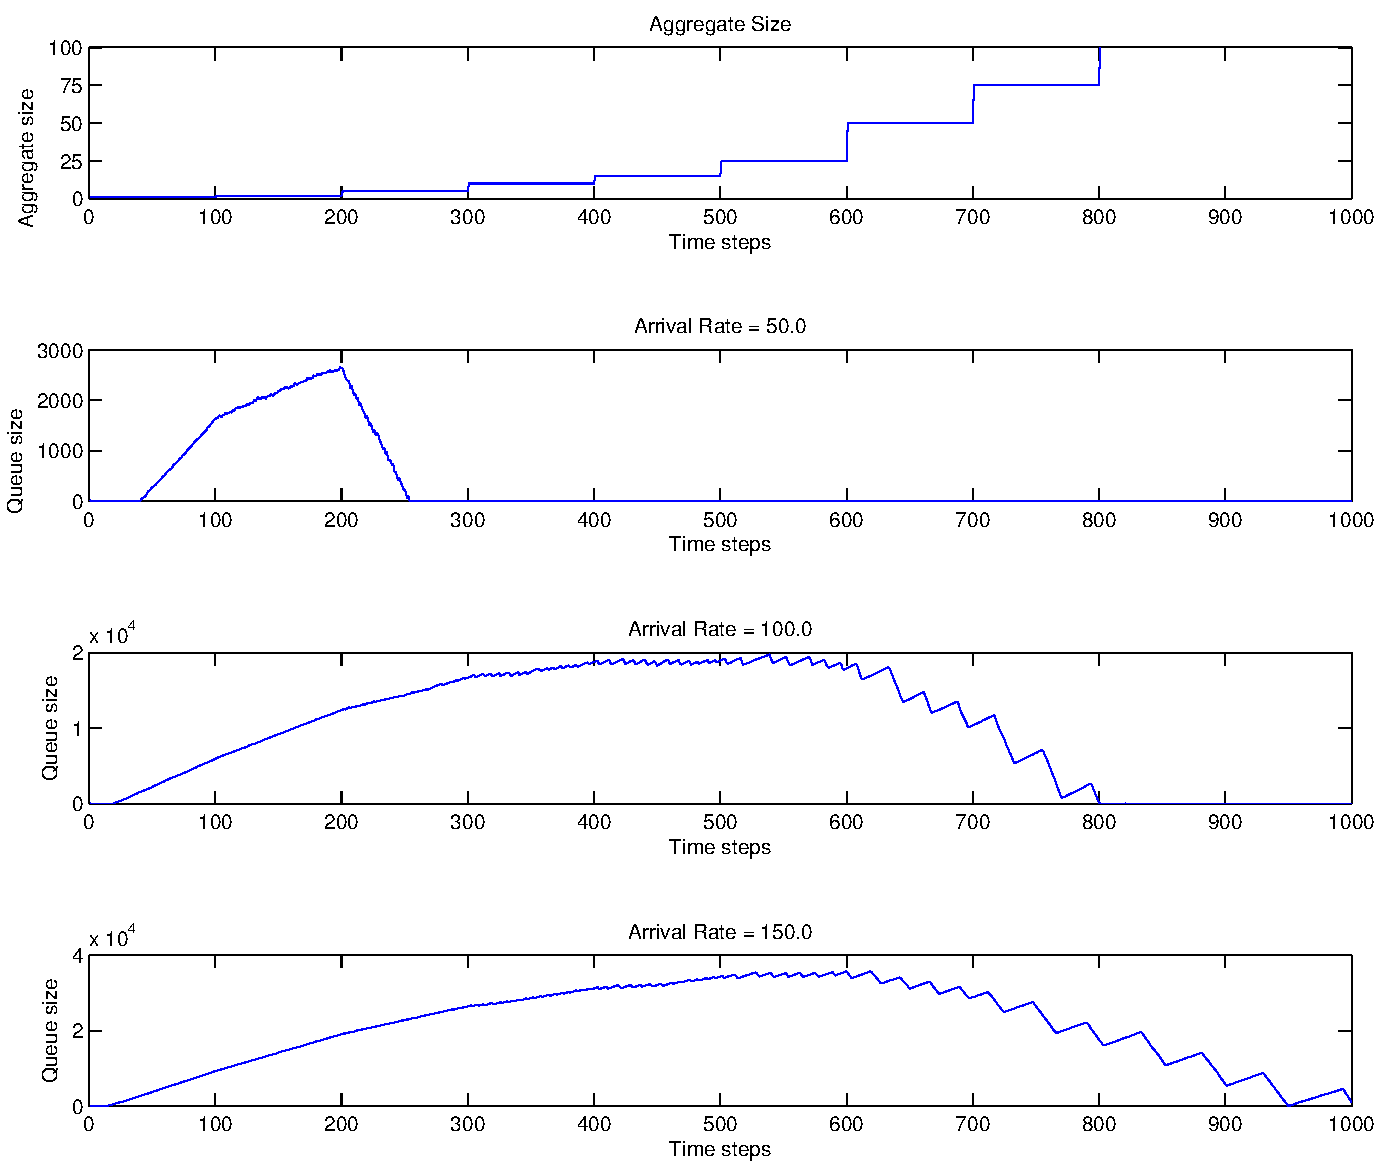
\includegraphics[width=\textwidth]{ch05_static_tests_queue_size}
	\caption{Static test: queue sizes}
	\label{fig:ch5_static_tests_queue_size}
\end{figure}

\begin{figure}[htpb]
	\centering
	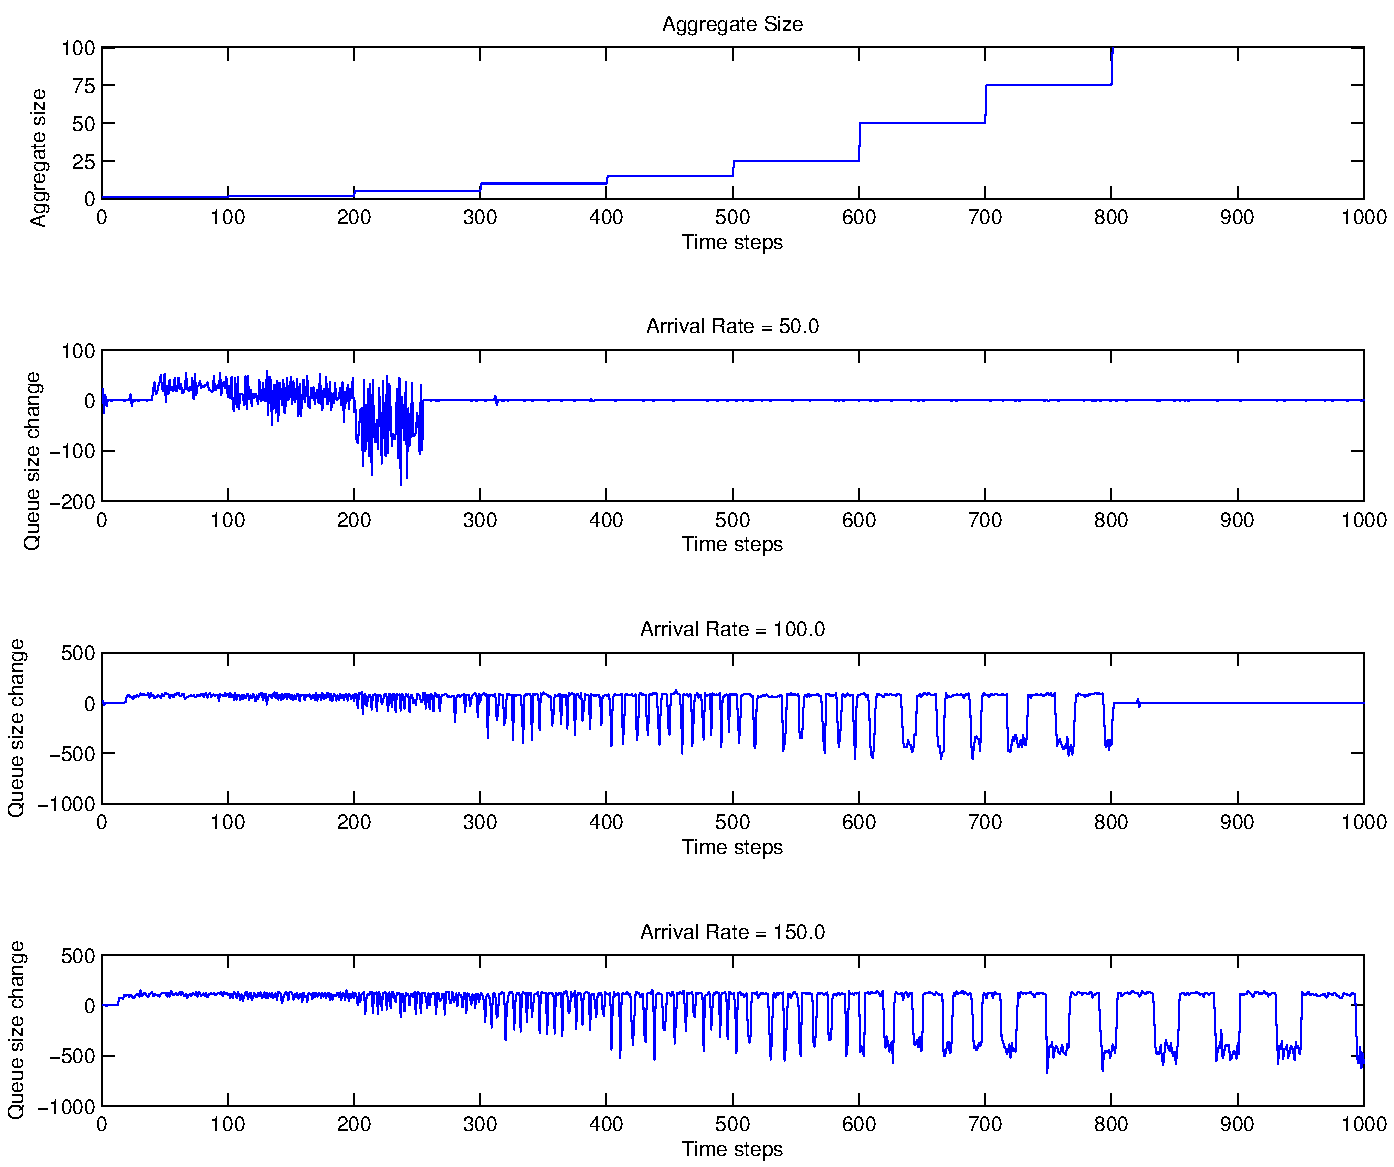
\includegraphics[width=\textwidth]{ch05_static_tests_queue_size_change}
	\caption{Static test: queue size changes}
	\label{fig:ch5_static_tests_queue_size_change}
\end{figure}

\subsubsection{Dynamic Tests}

The following test has been performed to evaluatate the performance of the \emph{Simple Controller}:

\begin{itemize}
	\item Events are generated with an $arrival\ rate = 50.0$ for 100 timesteps. 
	\item At $timestep = 100$, the arrival rate is set to 150.0 for another 100 timesteps. 
	\item At $timestep = 200$, the arrival rate is set back to 50.0.
\end{itemize}

Figure \ref{fig:ch5_dynamic_test_simple_controller} shows the results of this test using the \emph{Simple Control} strategy.

\begin{itemize}
	\item The controller is reasonably able to control the size of the queue. At $timestep = 100$, it increases the aggregate size to a maximum value of x. 
	\item At $timestep = 200$, the controller starts to decrease the aggregation size. At $timestep = 375$, the aggregation size is back at y.
\end{itemize}

\begin{figure}[htpb]
	\centering
	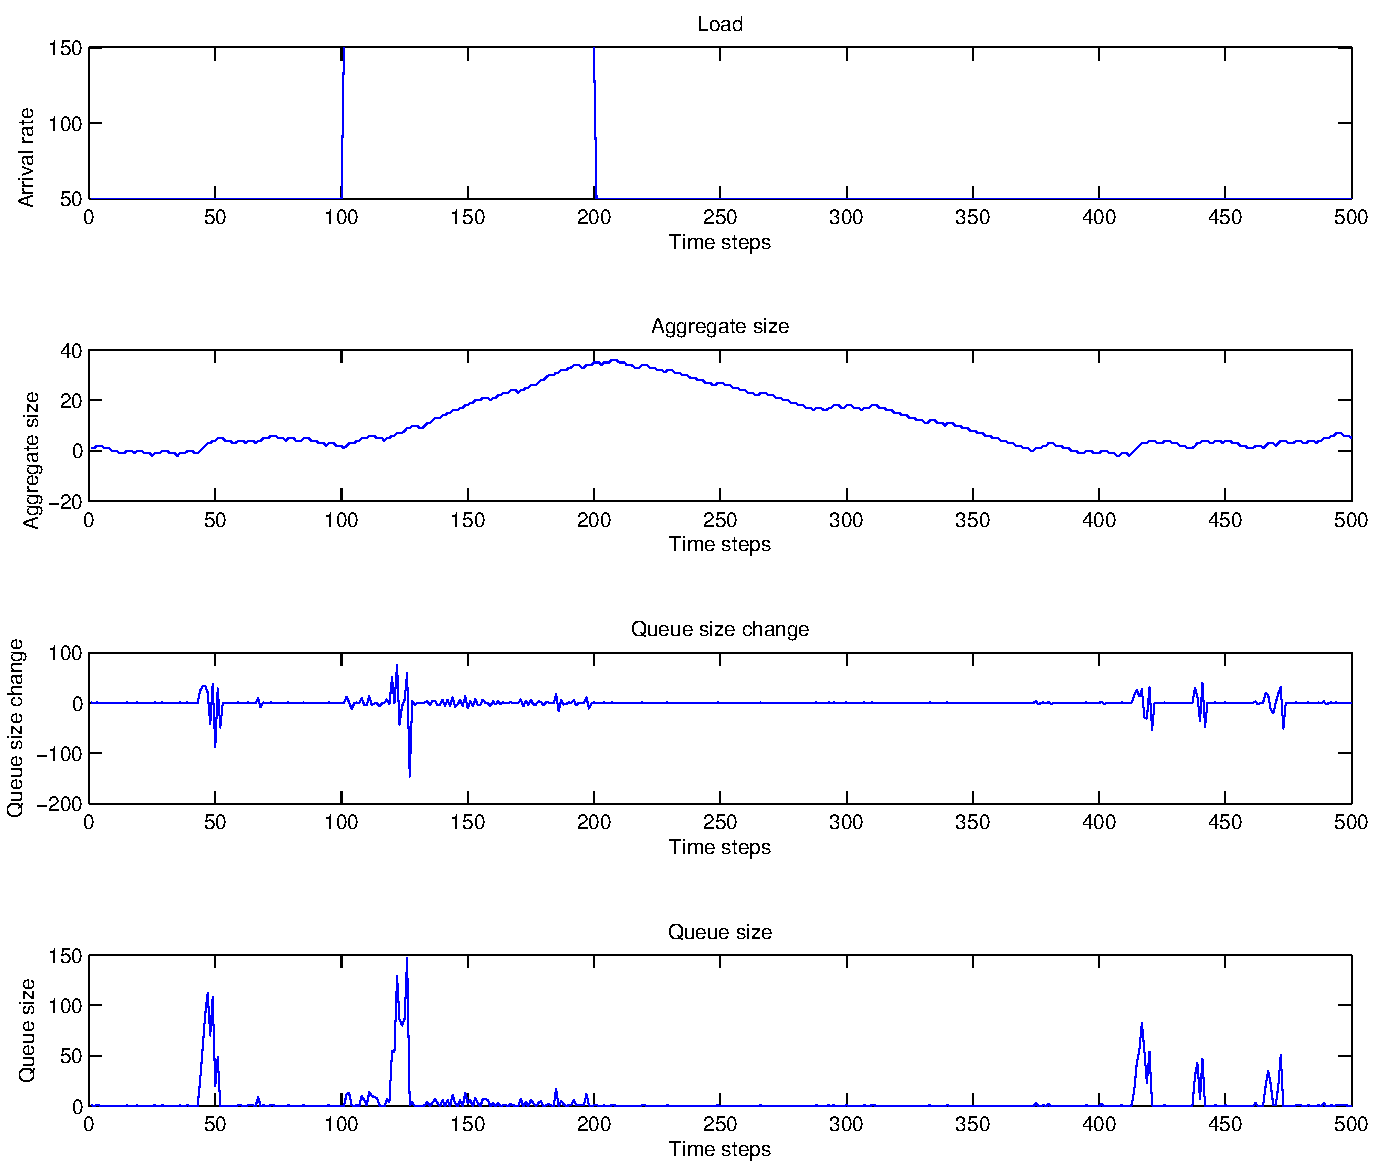
\includegraphics[width=\textwidth]{ch05_simple_controller}
	\caption{Simple control strategy}
	\label{fig:ch5_dynamic_test_simple_controller}
\end{figure}

\subsection{Results}

\section{Discussion with respect to related work}\label{sec:ch5_related_work}
This section gives an overview of work related to the adaptive middleware for bulk data processing presented in this chapter and discusses the approach that has been taken.

\subsection{Feedback Control of Computing Systems}

Feedback control is a common technique to implement 

\begin{itemize}
	\item General definition of Feedback Control
	\item Properties of Feedback Control Systems
	\item Open-Loop and Closed-Loop Control Systems
	\item Applications for Feedback Control
	\begin{itemize}
		\item Feedback-Control of Software Performance and \ac{QoS}
	\end{itemize}
\end{itemize}

\begin{itemize}
	\item Feedback Control of Computing Systems \citep{Hellerstein:2004a}
	\begin{itemize}
		\item Applications of Control Theory to Computing Systems
		\item Examples of Feedback Control Systems
	\end{itemize}
	\item Introduction to Control Theory And Its Application to Computing Systems \citep{Abdelzaher:2008ub}
	\item Challenges of Feedback Control of Computing Systems \citep{Hellerstein:2004tu}
	\item A Systematic Survey on the Design of Self-Adaptive Software Systems using Control Engineering Approaches \citep{Patikirikorala:2012ky}
	\item Control Systems application in Java based Enterprise and Cloud Environments \- A Survey \citep{Gullapalli:2011vn}
	\item Engineering Self-Adaptive Systems through Feedback Loops \citep{Brun:2009ww}
\end{itemize}

\begin{itemize}
	\item Feedback-Control of Software Performance and \ac{QoS}
	\begin{itemize}
		\item Feedback Performance Control in Software Services \citep{Abdelzaher:2003ea}
		\item ControlWare: A Middleware Architecture for Feedback Control of Software Performance \citep{Zhang:2002gf}
		\item Intelligent Enterprise Application Servers: A Vision for Self-Managing Performance \citep{Kumar:2013bw}
		\item Self-regulating Message Throughput in Enterprise Messaging Servers - A Feedback Control Solution \citep{Kumar:2012we}
	\end{itemize}
\end{itemize}

The \emph{Adaptive Middleware} presented in this chapter utilizes a closed-feedback loop to control the aggregation size of the processed messages, depending on the current load of the system. This is a novel approach that has not previously been investigated.

\section{Summary}\label{sec:ch5_summary}
In this paper, we have presented a middleware that is able to adapt itself to changing load scenarios by fluently shifting the processing type between single event and batch processing. The middleware uses a closed feedback loop to control the end-to-end latency of the system by adjusting the level of message aggregation depending on the current load of the system. Determined by the aggregation size of a messsage, the middleware routes a message to appropriate service endpoints, which are optimized for either single-event or batch processing.

To evaluate the proposed middleware concepts, we have implemented a prototype system and performed preliminary performance tests. The tests show that throughput and latency of a messaging system depend on the level of data granularity and that the throughput can be increased by increasing the granularity of the processed messages.

Next steps of our research are the implementation of the proposed middleware including the evaluation and tuning of different controller architectures, performance evaluation of the proposed middleware using the prototype and developing a conceptional framework containing guidelines and rules for the practitioner how to implement an enterprise system based on the adaptive middleware for near-time processing
